\section{Evaluation Strategies}
\label{sec:eval-strat}
As explained in \cref{ssec:supp-diff-ways}, there are multiple ways for
specifying the dynamic semantics of a language. Interpretation can for example
be performed through an interpreter generated from a DynSem specification, or by
implementing the interpreter in Stratego or Java. However, ultimately all of
these methods do the same thing. That is, they accept an AST as input and
somehow transform it into an output. In Spoofax, both the AST input and the
output value can be represented as a Stratego term. This is due to the fact that
the format for terms in Spoofax supports all of the basic types that Java has:
integers, real numbers, strings, lists and named constructor applications for
encoding objects~\cite{Brand00}. It is only the internal representation of an
interpreter's evaluation context and the implementation of the interpreter that
differs.

The strategy pattern is a pattern for encapsulating computation tasks that have
the same types of input and output, but a different implementation. This is
precisely the case for the different methods of evaluation: the method or
``strategy'' of evaluation is therefore put behind an interface called
\texttt{IEvaluationStrategy}. \Cref{fig:uml-eval-strat} shows a UML diagram
of this part of the design.

\begin{figure}[t]
  \centering
  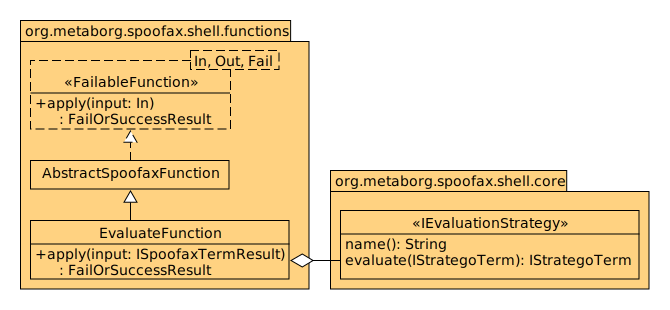
\includegraphics[width=0.8\textwidth]{uml-eval-strat}
  \caption{UML of the \texttt{IEvaluationStrategy} interface and its
    collaborators.}
  \label{fig:uml-eval-strat}
\end{figure}

An implementer of the \texttt{IEvaluationStrategy} is responsible for performing
evaluation on an AST representation of a program within the evaluation context
that it maintains throughout successive invocations. In this way, maintaining
the evaluation context is encapsulated, and no assumptions are made of what the
evaluation context looks like. This is a desirable property since the
representation of an evaluation context varies across languages and evaluation
methods.

%%% Local Variables:
%%% mode: latex
%%% TeX-master: "../main"
%%% End:
